% !Mode:: "TeX:UTF-8"
%% 请使用 XeLaTeX 编译本文.
%本模板在武汉大学硕士学位论文模板以及内蒙古科技大学硕士学位论文基础基础上修改，感谢原作者的工作！http://aff.whu.edu.cn/huangzh/ (武汉大学) and richey@imust.edu.cn (内蒙古科技大学)
%本模版联系方式wangxin2168@163.com
\documentclass[forprint]{XAUTPhD}   % 选项 
\addbibresource[location=local]{XAUTPhD.bib}

%%%%%%%%%%%%%%%%%%%%%%%%%%%%%%%%%%%%%%%%%%%%%%%%%%%%
\begin{document}

\CTitle{西安理工大学博士学位论文模板}     %论文题目中文名
\CTitleFirstLine{~ 西安理工大学博士学位论文 ~}   %论文题目中文名分行一行
\CTitleSecondLine{~ 模板模板 ~}                  %论文题目中文名分行二行

\StudentAuthor{王鑫}                %姓名
\StudentNumber{1220000000}          %学号
\Csupervisor{刘龙}                  %指导教师中文名
\CsupervisorTitle{教授}             %指导教师职称
\Cmajor{控制科学与工程}              % 学科（领域）名称
\CSchool{自动化与信息工程学院}        %学院
\CUniversity{西安理工大学}           %学校
\ClassficationNumber{ TP182  }     %分类号
\SecretLevel{~~~公开~~~}            %密级
\UDC{\quad\quad\quad ~}            %UDC
\UniversityCode{10700}             %学校代码
\DegreeCategory{工学}               %学位类别
\AssistSupervistor{赵建敏}          %协助指导教师
\AssistSupervistorTitle{副教授}     %协助指导教师职称
\PaperDate{2020年6月10日}           %目前为自动获取当日日期，若需手动可设置此参数

\ETitle{XI'AN UNIVERSITY OF TECHNOLOGY DOCTORAL DISSERTATION TEMPLATE}     
                                              %论文题目英文名
\Emajor{Control Science and Engineering}      % 学科英文名称
\EStudentAuthor{Xin Wang}                     % 英文名
\Esupervisor{Long Liu}                        %指导教师英文名
\EsupervisorTitle{Prof.}                      %指导教师英文职称

%%%============= 封面 ============%%%-------------------------------------------
\pdfbookmark[0]{封面}{title}         % 封面页加到 pdf 书签
\pagenumbering{gobble} 
% !Mode:: "TeX:UTF-8"
% pages/coverpage.tex
%%%--- “封面” --- %%%%%%%%%%%%%%%%%

\thispagestyle{empty}%

% 书脊
\printCoverBox{0.8cm}{-3.8cm}{2.05cm}{-26.8cm}{0.25mm}

\begin{textblock}{1}[0,0](0.2, 3)
    \zihao{4}\songti
    \begin{minipage}[t][24.3cm][c]{0.5em} %\textheight
        \printSpine
    \end{minipage}
\end{textblock}

% 特殊信息
\begin{textblock}{6}(12.75,3.45) % 宽度Zcm，位置(Xcm,Ycm)
    \zihao{-4}\songti
    \renewcommand{\arraystretch}{0.85}
    \begin{tabular}{|p{1.8cm}|p{2.45cm}|}
        \hline
        \makebox[1.8cm][s]{分类号}    & \the\ClassficationNumber \\
        \hline
        \makebox[1.8cm][s]{学校代码}  & \the\UniversityCode \\
        \hline
        \makebox[1.8cm][s]{学号}     & \the\StudentNumber \\
        \hline
    \end{tabular}
\end{textblock}

\begin{center}
    \vspace{170pt}
    
\includegraphics[width=8.53cm,height=1.53cm]{xaut01.png} %%
    \vspace{23pt}
    
    {\heiti\fontsize{48pt}{48pt}\bfseries{
    博士学位论文
    }}
    
    \vspace{50pt}
    % \hspace{44pt}
    {\zihao{-3}\songti
        \renewcommand\arraystretch{1.2}
        % \hspace{4cm}
        \begin{tabular}{c}
            \songti\zihao{3}\bfseries{\thickuline{\makebox[18em]{\the\CTitleFirstLine}}} \\
            \songti\zihao{3}\bfseries{\thickuline{\makebox[18em]{\the\CTitleSecondLine}}} \\
        \end{tabular}\\
    }
    {\zihao{-3}\songti
    \vspace{2\baselineskip}
    }

    {
    \songti\zihao{-3}\bfseries{\thickuline{~~\the\StudentAuthor ~~~}}
    }
    
    \vspace{65pt}
    % \hspace{44pt}
    {\zihao{-3}\songti
        \renewcommand\arraystretch{1.35}
        %\hspace{1.4cm}
        \begin{tabular}{lccc}
            \makebox[6em][s]{\textbf{学科门类:}} & \multicolumn{3}{c}{\thickuline{\makebox[12.5em]{\textbf{\the\DegreeCategory}}}} \\
            \makebox[6em][s]{\textbf{学科名称:}}
            & \multicolumn{3}{c}{\thickuline{\makebox[12.5em]{\textbf{\the\Cmajor}}}} \\
            \makebox[6em][s]{\textbf{所在学院:}}
            & \multicolumn{3}{c}{\thickuline{\makebox[12.5em]{\textbf{\the\CSchool}}}} \\
            \makebox[6em][s]{\textbf{指导教师:}}
            & \multicolumn{3}{c}{\thickuline{\makebox[12.5em]{\textbf{\the\Csupervisor~~\the\CsupervisorTitle}}}} \\
            \makebox[6em][s]{\textbf{申请日期:}}
            & \multicolumn{3}{c}{\thickuline{\makebox[12.5em]{\textbf{\today}}}} \\
        \end{tabular}		
    }
\end{center}%

\cleardoublepage             % 加入封面.

%%%=========== 独创性声明 =========%%%-------------------------------------------
% !Mode:: "TeX:UTF-8"
% pages/originalitystate.tex
%%%--- “独创性说明” --- %%%%%%%%%%%%%%%%%

\clearpage
\pagestyle{empty}
\newpage
\newgeometry{left=2.8cm, right=2.2cm, top=3cm, bottom=3cm}
\vspace*{20pt}
\begin{center}{\ziju{0.5}\zihao{-1}\songti\bfseries 独创性声明}\end{center}
\par\vspace*{25pt}
\renewcommand{\baselinestretch}{1.5}

{\zihao{-4} \songti \bfseries

本人所呈交的学位论文是在导师指导下进行的研究工作及取得的成果。尽我所知，除特别加以标注的地方外，论文中不包含其他人的研究成果。与我一同工作的同志对本 文的研究工作和成果的任何贡献均已在论文中作了明确的说明并已致谢。

本论文及其相关资料若有不实之处，由本人承担一切相关责任。

\vspace*{25pt}
\begin{flushright}
论文作者签名：\underline{\hspace{2.3cm}}\hspace{2cm}年\hspace{0.8cm}月\hspace{0.8cm}日
\end{flushright}

%%%%%%%-------------------------------------------------

%%%%%%%-------------------------------------------------
%%%--- 加入``授权声明'' --- %%%%%%%%%%%%%%%%%

\vspace*{88pt}
\begin{center}{\ziju{0.1}\zihao{2}\songti\bfseries 学位论文使用授权}\end{center}
\par\vspace*{34pt}
% \renewcommand{\baselinestretch}{1.5}

\zihao{-4} \songti %

本人作为学位论文作者了解并愿意遵守学校有关保留、使用学位论文的规定，即：在导师的指导下创作完成的学位论文的知识产权归西安理工大学所有，本人今后在使用或发表该论文涉及的研究内容时，会注明西安理工大学。西安理工大学拥有学位论文的如下使用权，包括：学校可以保存学位论文；可以采用影印、缩印或其他复制手段保存论文；可以查阅或借阅。本人授权西安理工大学对学位论文全部内容编入公开的数据库进行检索。本学位论文全部或部分内容的公布（包括刊登）授权西安理工大学研究生院办理。
\vspace*{15pt}

涉密的学位论文按照《西安理工大学研究生学位论文涉密认定和管理办法》要求进行密级认定，学校按照密级对学位论文进行分类管理。

保密的学位论文在解密后，适用本授权。

\vspace*{42pt}

\begin{flushright}
论文作者签名：\underline{\hspace{2cm}}\hspace{1cm}导师签名：\underline{\hspace{2cm}}\hspace{2cm}年\hspace{0.8cm}月\hspace{0.8cm}日
\end{flushright}
}
\cleardoublepage % 结束当前页
\restoregeometry % 恢复之前的页边距设置      % 加入独创性声明.

%%%=========== 中英文摘要 =========%%%-------------------------------------------
\pagenumbering{Roman}               % 正文之前的页码用大写罗马字母编号.
\pagestyle{frontplain}
% !Mode:: "TeX:UTF-8"
% pages/abstract.tex

%%%--- “中文摘要” --- %%%%%%%%%%%%%%%%%

% \pagestyle{plain}
% \newpage
% \newpage  \pagestyle{plain} \myplain
% \newgeometry{left=2.6cm, right=2.1cm, top=2.5cm, bottom=2.1cm, includefoot}
% \linespread{1.25}

\begin{flushleft}
{\zihao{3}\heiti
    \makebox[5em][s]{\textbf{论文题目：}}\textbf{\the\CTitle}\\
    \makebox[5em][s]{\textbf{专业名称：}}\textbf{\the\Cmajor}\\
    \makebox[5em][s]{\textbf{研究生：}}\textbf{\the\StudentAuthor}\hfill \makebox[3.5em][s]{\textbf{签名：}}\thickuline{\quad\quad\quad\quad\quad\quad}\\
    \makebox[5em][s]{\textbf{指导老师：}}\textbf{\the\Csupervisor~~\the\CsupervisorTitle}\hfill \makebox[3.5em][s]{\textbf{签名：}}\thickuline{\quad\quad\quad\quad\quad\quad}\\
}
\end{flushleft}

\begin{cnabstract}
博士学位论文摘要是对论文研究内容、方法与主要成果的高度概括，是读者了解论文核心贡献的重要部分。摘要应能够在不阅读全文的情况下，使读者清晰了解研究问题、研究方法及主要结论。一般而言，博士论文摘要应包括以下几个方面的内容。研究背景与问题提出：简要介绍研究领域的发展背景及存在的关键问题，说明本研究开展的必要性与研究意义。该部分应突出研究问题，而不宜进行过多的文献综述；研究目标与研究内容：概述论文的主要研究目标，并简要说明论文围绕该目标开展的核心研究内容或研究思路；研究方法与技术路线：介绍论文所采用的主要研究方法、理论模型或技术框架，使读者能够理解研究工作的基本思路与方法特点；主要研究成果与创新点：重点概括论文取得的主要研究成果，包括提出的新方法、新模型或新理论，并突出论文的创新性贡献；结论与应用价值：简要总结研究结论，并说明研究成果的理论意义或实际应用价值。

在写作形式上，摘要应具有独立性和完整性，避免使用“本文”“本章”等指代性较强的表达，同时一般不引用文献、不出现图表和公式。摘要内容应逻辑清晰、语言精炼，通常控制在 800–1200 字左右（中文摘要）。摘要之后应给出 3–5 个关键词（Keywords），用于反映论文研究的核心主题。关键词应尽量选用学科领域内通用、规范的术语，并按照重要程度进行排列。

\par\vspace{\baselineskip}
\cnkeywords{博士学位论文；论文模板；格式规范；图表使用；附件引入}
\end{cnabstract}

\cleardoublepage % 结束当前页
% \restoregeometry % 恢复之前的页边距设置

%%%--- “英文摘要” --- %%%%%%%%%%%%%%%%%

\begin{flushleft}
{
\renewcommand{\baselinestretch}{1}
\zihao{4}\textsf{\textbf{Title: \the\ETitle}\\
    \vspace*{14pt}
    \textbf{Major: \the\Emajor}\\
    \vspace*{14pt}
    \textbf{Name: \the\EStudentAuthor}\hfill \textbf{Signature:} \thickuline{\quad\quad\quad\quad\quad\quad}\\
    \vspace*{14pt}
    \textbf{Supervisor: \the\EsupervisorTitle~~\the\Esupervisor}\hfill \textbf{Signature:} \thickuline{\quad\quad\quad\quad\quad\quad}\\
}}
\end{flushleft}

\begin{enabstract}

The doctoral dissertation abstract provides a concise summary of the thesis's research content, methodology, and primary findings, serving as a crucial component for readers to grasp the core contributions of the work. It should enable readers to clearly understand the research question, methodology, and main conclusions without reading the full text. Generally, a doctoral dissertation abstract should include the following elements. Research Background and Problem Statement: Briefly introduce the developmental context of the research field and the key existing problems, explaining the necessity and significance of this study. This section should highlight the research question without excessive literature review; Research Objectives and Content: Outline the primary research objectives and briefly describe the core research content or approach developed around these objectives; Research Methods and Technical Approach: Introduce the primary research methods, theoretical models, or technical frameworks employed, enabling readers to grasp the fundamental methodology and methodological characteristics of the work. Key Findings and Innovations: Summarize the main research outcomes, including novel methods, models, or theories proposed, emphasizing the innovative contributions of the thesis. Conclusions and Practical Value: Briefly summarize the research conclusions and articulate the theoretical significance or practical application value of the findings.

In terms of writing format, the abstract should be self-contained and complete, avoiding highly referential expressions such as “this paper” or “this chapter.” Generally, it should not cite references, include figures or tables, or present mathematical formulas. The abstract should be logically coherent and concisely written, typically limited to 800–1200 words (for Chinese abstracts). Following the abstract, provide 3–5 keywords (Keywords) reflecting the core themes of the paper's research. Keywords should prioritize standardized terminology within the discipline and be listed in order of importance.

\par\vspace{\baselineskip}
\enkeywords{Doctoral Dissertation; Dissertation Template; Formatting Guidelines; Use of Figures and Tables; Inclusion of Appendices}
\end{enabstract}

\cleardoublepage % 结束当前页
% \restoregeometry % 恢复之前的页边距设置              % 加入中英文摘要

%%%============= 目录 ============%%%-------------------------------------------
\pdfbookmark[0]{目录}{toc}          % 把目录加入到书签
\tableofcontents

%%%%%%%%%%%%%%%%%%%%%%%%%%%%%%%%%%%%%%%%%%%%%%%%%%%%%%%%%%%%%%%%%%%%%%%%%%%%%%%
\newpage \pagestyle{fancyfancyfancy} \fancyfancy
\mainmatter %% 以下是正文
\baselineskip=20pt  % 正文行距为 20 磅

%%%============= 正文 ============%%%-------------------------------------------
% !Mode:: "TeX:UTF-8"

\chapter{绪论}
\section{研究背景与意义}
\subsection{研究背景}

在博士学位论文中，研究背景通常采用分段方式逐层展开，从宏观领域到具体研究问题，逻辑上逐步收敛。一般可以分为 3–4 个自然段进行描述，每一段承担不同的功能。

首先介绍研究领域的发展趋势和研究意义，从宏观层面说明该研究方向的重要性。该段应当突出研究领域的应用价值或学术价值，使读者了解研究问题所处的大背景。如：随着人工智能与计算机视觉技术的快速发展，智能感知与行为理解逐渐成为计算机视觉领域的重要研究方向。人体动作分析作为其中的关键任务，在智能监控、人机交互、虚拟现实以及医疗康复等领域具有广泛应用价值。通过对人体动作的准确建模与理解，能够有效提升智能系统对复杂场景的感知能力，因此受到了学术界和工业界的广泛关注。

在宏观背景基础上，进一步聚焦到具体研究对象或研究任务，并说明其研究特点或优势。如：在人体行为理解研究中，基于骨骼数据的动作表示由于能够直接反映人体关节的空间结构信息，同时对外观变化和背景干扰具有较强鲁棒性，近年来逐渐成为研究热点。与传统基于RGB视频的方法相比，骨骼数据具有结构清晰、维度较低等特点，使其更适合进行人体动作的时空建模。然而，骨骼动作序列通常包含复杂的空间拓扑关系和时间动态变化，如何有效建模其时空依赖关系仍然是一个具有挑战性的研究问题。

进一步介绍目前主流研究方法，并指出其存在的不足，从而引出研究问题。如：现有研究主要采用卷积神经网络、图卷积网络以及Transformer等深度学习模型对骨骼动作进行建模。其中，图卷积网络能够利用人体骨骼的拓扑结构信息，在动作识别任务中取得了较好的效果。然而，这类方法在建模长程时空依赖关系以及复杂动作动态变化方面仍存在一定局限。此外，在动作生成任务中，传统生成模型在生成稳定性和动作真实性方面仍面临挑战。因此，探索更加有效的人体动作建模与生成方法仍具有重要研究意义。

\subsection{研究意义}

研究意义主要用于说明本研究开展的价值与贡献，通常从 理论意义 和 实际应用意义 两个方面进行阐述。通过研究意义的描述，可以进一步突出论文研究工作的必要性和重要性。

随着移动互联网以及人工智能的发展，人类社会已经进入了数字化、信息化和智能化的时代。而计算机视觉技术作为分析和处理海量数据的关键技术，已在深度学习领域发挥出了巨大效用。人是大量视觉数据的主要目标，人体行为是实现目的、欲望、意识和意志等的主要手段，是人的一种重要的社会属性，如图\ref{fig:applications}所示。

\begin{figure}[htbp]
    \centering
    \begin{subfigure}[b]{0.4\textwidth}
        \centering
          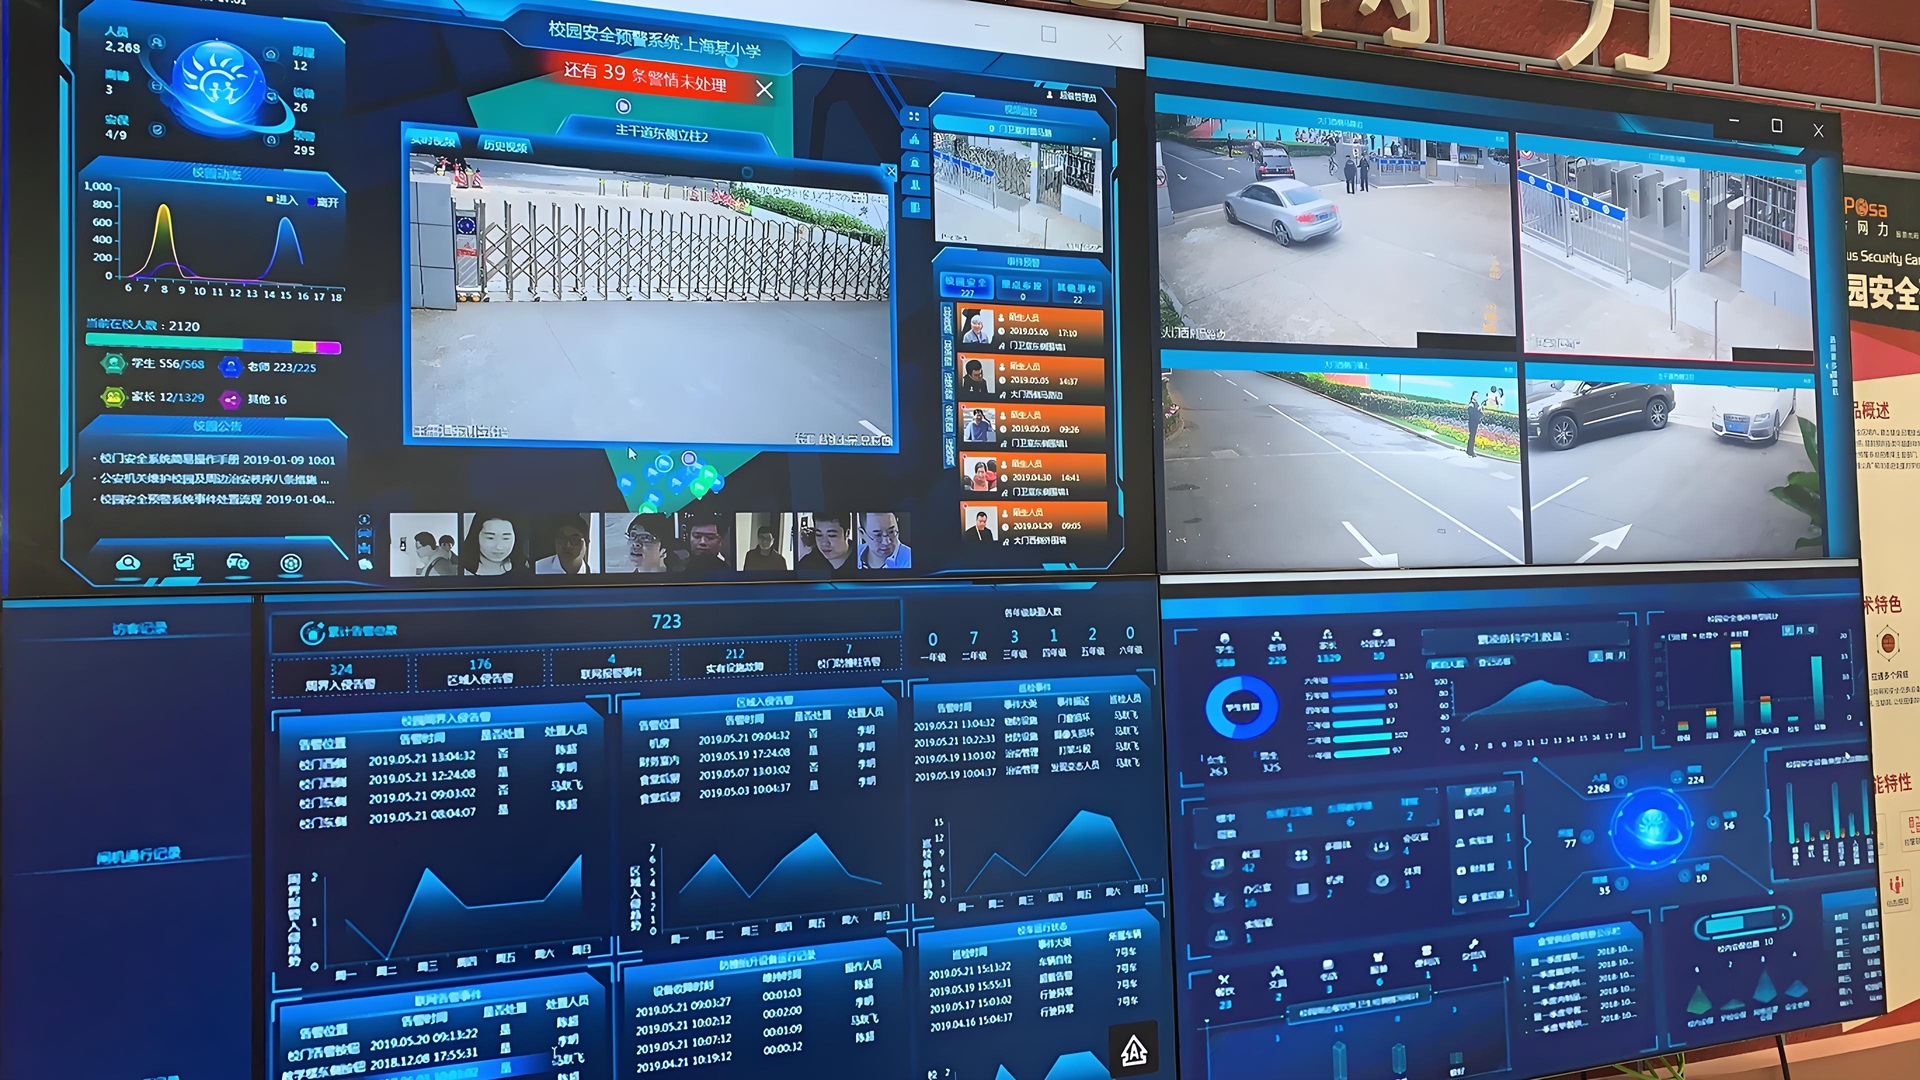
\includegraphics[width=\linewidth]{figures/Fig1a.jpg}
        \caption{安防监控}
    \end{subfigure}
    \hspace*{15pt}
    \begin{subfigure}[b]{0.4\textwidth}
        \centering
        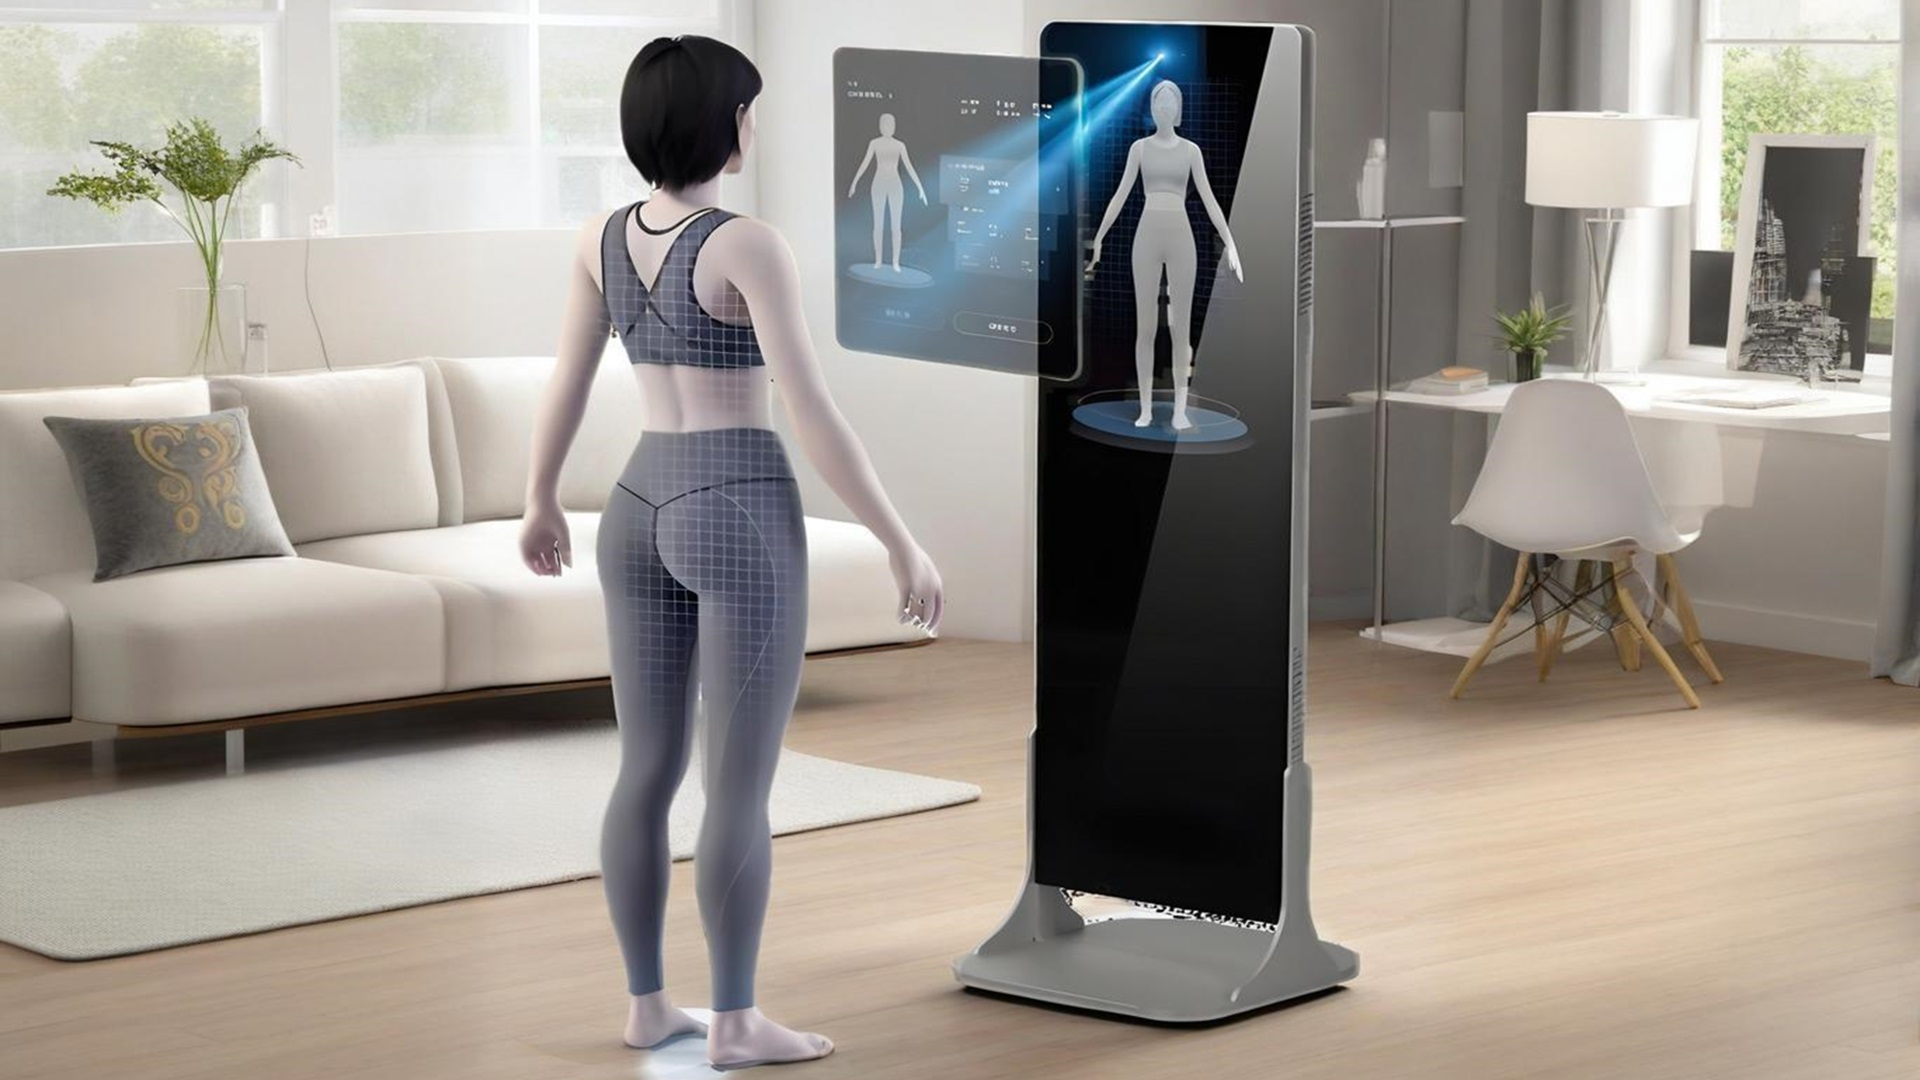
\includegraphics[width=\linewidth]{figures/Fig1b.jpg}
        \caption{智能家居}
    \end{subfigure}
    \\
    \begin{subfigure}[b]{0.4\textwidth}
        \centering
        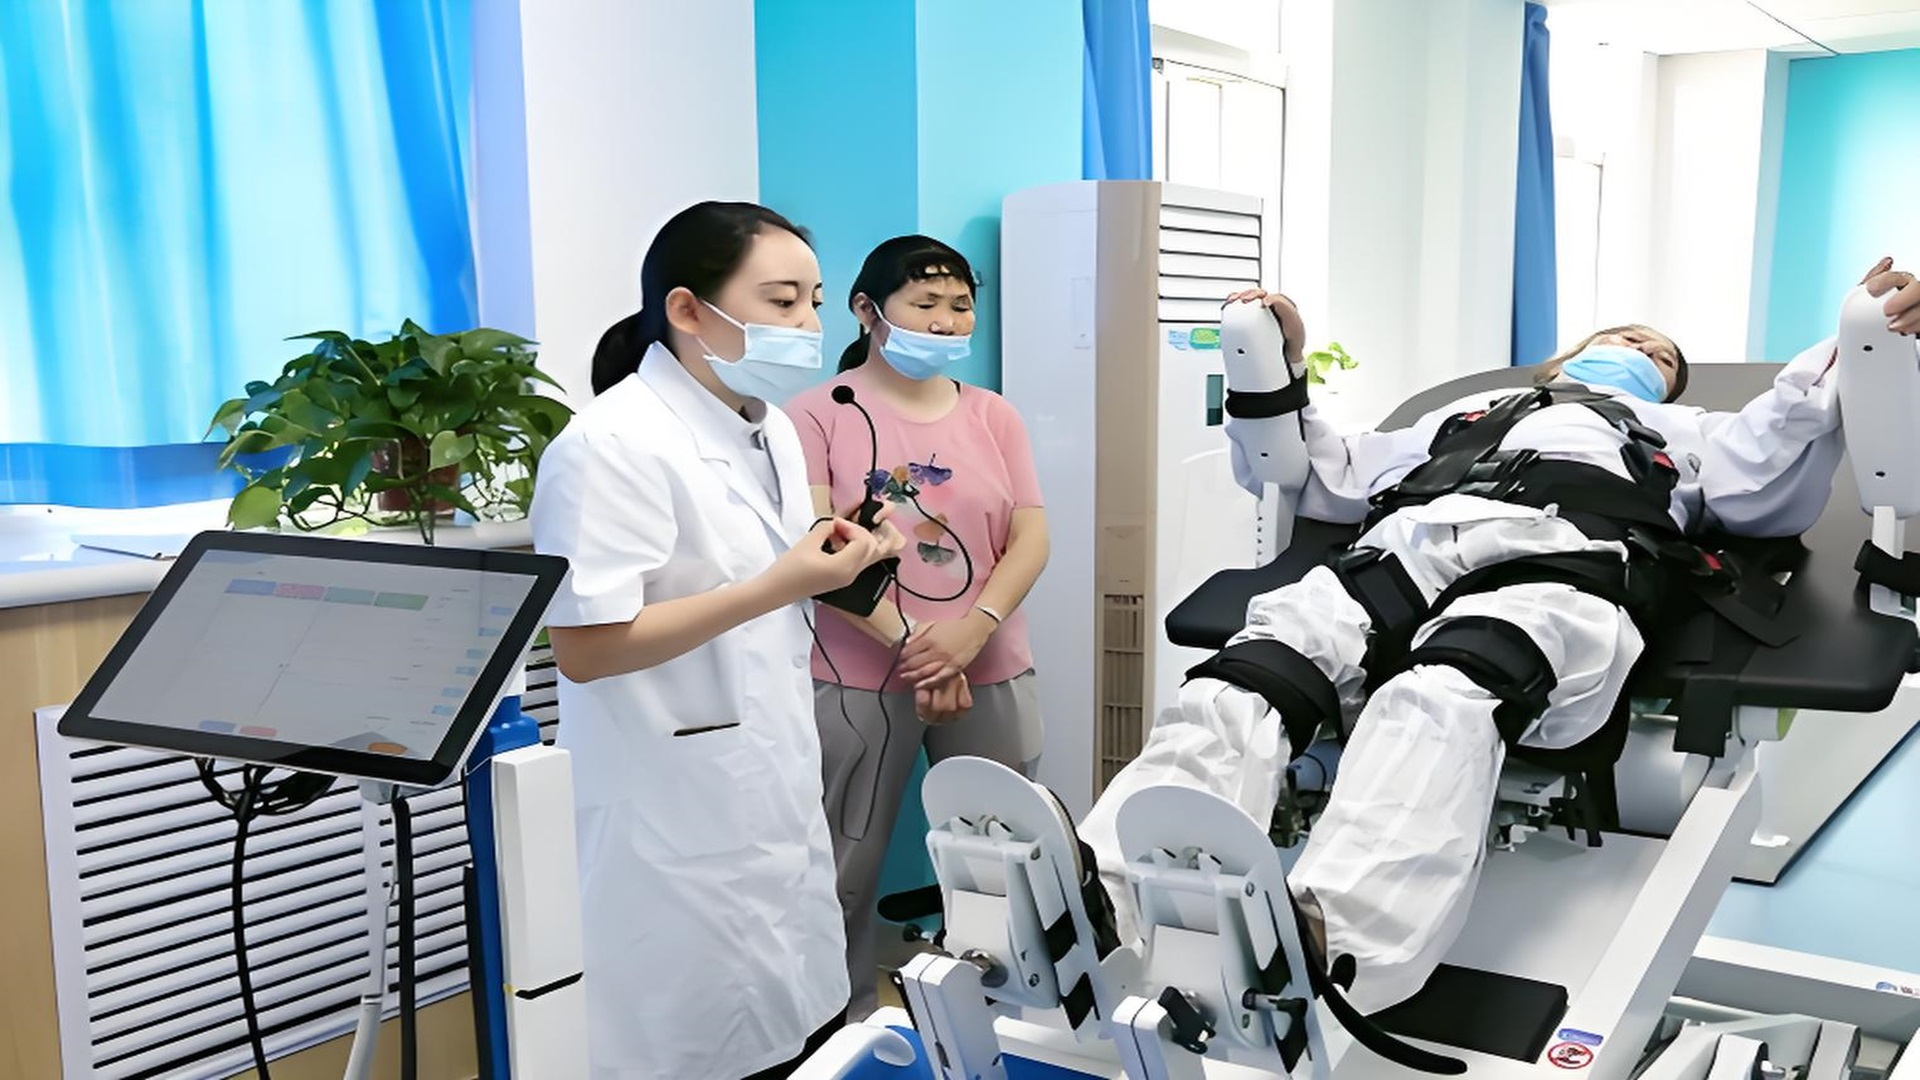
\includegraphics[width=\linewidth]{figures/Fig1c.jpg}
        \caption{医疗康复}
    \end{subfigure}
    \hspace*{15pt}
    \begin{subfigure}[b]{0.4\textwidth}
        \centering
        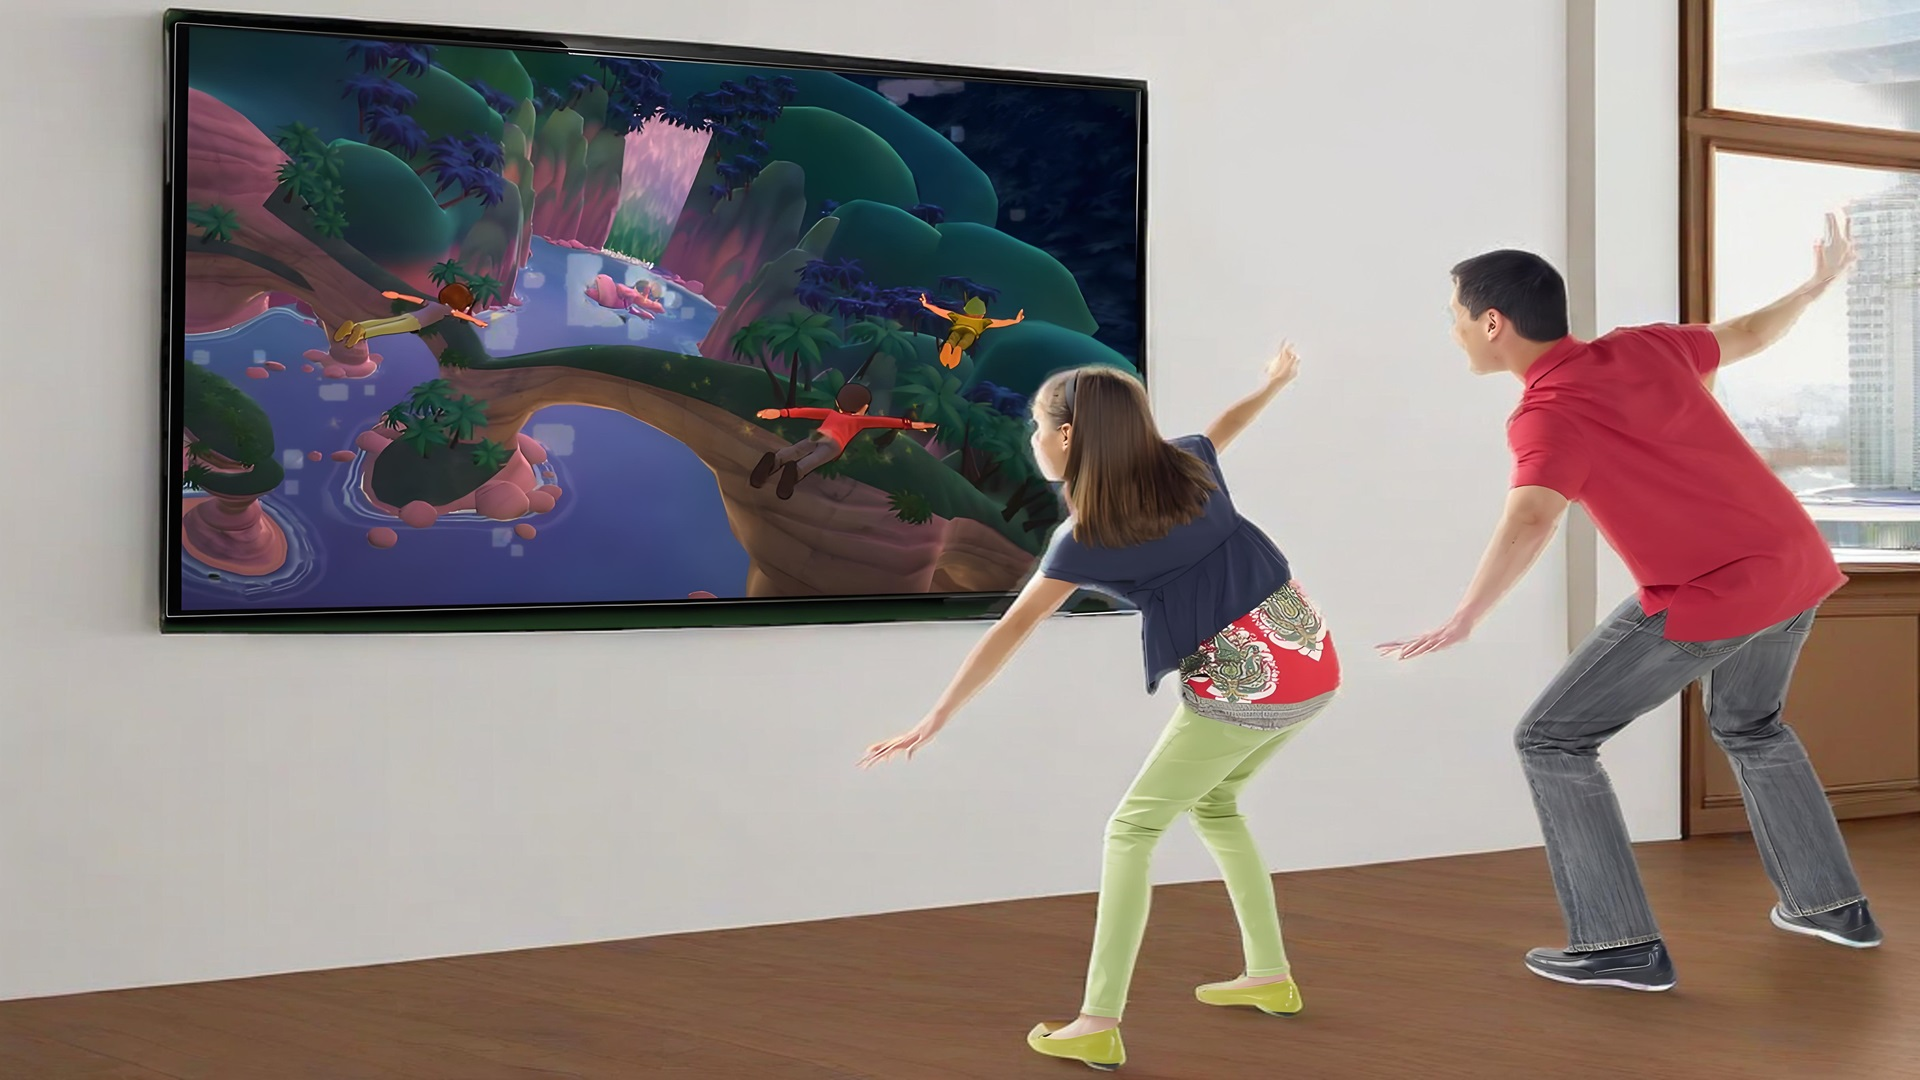
\includegraphics[width=\linewidth]{figures/Fig1d.jpg}
        \caption{人机交互}
    \end{subfigure}
\bilingualfigure{人体行为分析应用领域}{Applications of human action Analysis}
\label{fig:applications}
\end{figure}

\section{国内外研究现状}

在博士论文绪论中，“国内外研究现状”部分主要用于系统梳理该领域已有研究成果，并指出现有研究的不足，从而为论文研究内容提供依据。该部分通常采用分段或分小节的方式进行论述，按照研究方向或技术路线进行分类介绍，而不是简单罗列文献。

\subsection{XXX国内外现状}

\subsection{XXX国内外现状}

\subsection{XXX国内外现状}

\section{拟解决的关键问题}

在博士学位论文绪论中，“拟解决的关键问题”部分主要用于明确论文研究所要突破的核心问题，是从前面的研究现状与不足自然过渡而来的。该部分通常不需要很长，但需要概括准确、逻辑清晰、突出问题本质。一般可先用一段总体说明，然后以条目式或分段方式列出若干关键问题。

\section{本文研究内容}

在博士论文绪论中，“本文研究内容”部分主要用于概括论文开展的具体研究工作。该部分通常在“拟解决的关键问题”之后，通过条目式或分段方式介绍论文的主要研究内容，使读者能够清晰了解论文各项研究工作的整体结构。一般先给出一段总体说明，然后列出 3–5 项具体研究内容。

\section{本文组织结构}

在博士学位论文绪论中，“本文组织结构”部分主要用于介绍论文各章节的安排，使读者能够快速了解论文整体结构与内容分布。该部分通常采用一段总述 + 分章节说明的写法，对每一章的主要内容进行简要概括。
% !Mode:: "TeX:UTF-8"

\chapter{视觉文本描述基础(测试)}
视觉文本描述是跨机器视觉和自然语言处理领域的一个挑战性课题。在描述视觉内容的过程中，通过机器视觉中的特征提取模块，将输入图像或视频转化为计算机所能理解的形式，再通过自然语言处理将视觉内容转化为自然语言的形式。在转化过程中，需要确保描述内容与视觉内容的一致性(即语义对齐)。本章介绍了视觉文本描述中常用的基本概念、理论，主要包括视觉特征提取、自然语言生成、常见的语义对齐方法、损失函数、通用标准测试集以及评价指标。从而为后续章节的算法研究奠定理论基础。

\section{视觉特征提取(测试)}
视觉特征提取是视觉文本描述中至关重要的一步。心理学的研究表明，人们可以利用整幅图像内容理解视觉内容，也可以利用图像中物品的种类和关系对视觉内容进行理解。全局特征包含完整的图像信息，但也会含有大量无关信息，比如背景信息、非重要物品信息，同时，全局特征更容易受到光照、遮挡、噪声和多视角等的影响，导致泛化能力较弱。与之相反，局部的物品特征减少了无关信息的干扰，但往往缺少物品间的空间关系信息。场景图特征在局部特征的基础上添加了物品间的关系信息。时序特征则反应了视频中的时序信息。下面将分别介绍全局特征、局部特征、场景图特征以及时序特征。

\subsection{图像全局特征(测试)}
早期的图像文本描述常采用手工特征，例如：尺度不变特征变换(Scale-invariant feature transform, SIFT)[121]、方向梯度直方图(Histogram of Oriented Gradient, HOG)[122]、颜色直方图特征、Gabor特征和空间包络特征(Gist)[122]等。

由于手工特征准确率较低且缺乏扩展能力，当前的图像文本描述方法常通过基于深度学习的方法提取全局特征。基于深度学习的特征提取模型，是将原始图像的像素值输入模型中进行学习，生成隐含图像语义的特征。该方法最大的优点在于具有鲁棒性和普适性，只需要输入图像和对应标签，模型会自动进行学习，中间无需人为干扰，提取到的特征具有更强大的表达能力，是手工特征所无法达到的。

\subsection{图像局部特征(测试)}
早期的图像文本描述常采用手工特征，例如：尺度不变特征变换(Scale-invariant feature transform, SIFT)[121]、方向梯度直方图(Histogram of Oriented Gradient, HOG)[122]、颜色直方图特征、Gabor特征和空间包络特征(Gist)[122]等。

由于手工特征准确率较低且缺乏扩展能力，当前的图像文本描述方法常通过基于深度学习的方法提取全局特征。基于深度学习的特征提取模型，是将原始图像的像素值输入模型中进行学习，生成隐含图像语义的特征。该方法最大的优点在于具有鲁棒性和普适性，只需要输入图像和对应标签，模型会自动进行学习，中间无需人为干扰，提取到的特征具有更强大的表达能力，是手工特征所无法达到的。

\section{度量学习相关理论(测试)}

\section{数据集及评价指标(测试)}

\section{本章小结(测试)}
% !Mode:: "TeX:UTF-8"

\chapter{基于度量学习的视觉 3D 人体姿态估计方法(测试)}

\section{引言(测试)}
本研究针对现有人体姿态估计模型在实际应用中因环境复杂多变导致的泛化性不足问题，尝试了基于度量学习的视觉 3D 人体姿态估计方法。传统方法通过增加模型复杂度或扩充数据集提升指标性能，但面临两个核心矛盾：(1) 3D 标注数据获取成本高昂；(2)预训练模型难以适应新环境条件。本研究的创新性在于，基于已训练完成的 2D 姿态估计模型，通过引入新环境参考图像构建域适应机制，使模型无需重新训练即可快速适应不同光照、背景等环境变量，直接输出适配当前场景的 2D 姿态结果。最终结合三角测量方法实现 3D 关节坐标推算，本章的整体网络架构如图 3-1 所示。本章在实验环节，通过消融实验证明了参考视图个数对 2D 估计结果的影响，以及引入的图卷积结构的有效性，并在两个数据集中对比了本论文方法与其他方法的性能。

\section{基于度量学习的多视角 2D 人体姿态估计(测试)}
本节将介绍 2D 姿态估计环节的各个模块，首先介绍用于初步提取关节特征的网络，为了在 2D 阶段充分利用图像中的语义信息，本文选用 Swin Transformer[79]作为特征提取网络，分别提取待估计视图和参考视图中的关节特征。其次介绍相似性度量网络及其注意力热图的表现形式，最后介绍图卷积结构和特征解码结构。本节的 2D 姿态估计网络结构如图所示，在本节的最后，会给出该网络架构对应的实验结果与分析。

\subsection{特征提取网络(测试)}
随着 Alexnet 卷积神经网络在图像领域取得重大突破后，各类卷积神经网络也呈现爆发式增长，在人体姿态估计领域中，由于人体目标的尺度不一样，为了让模型能分辨不同尺度的人体目标，有些研究人员也考虑到对不同分辨率的人体图像做处理，提升模型的鲁棒性，使其能适应不同尺度的人体目标图像。

\subsection{特征编码结构(测试)}
随着 Alexnet 卷积神经网络在图像领域取得重大突破后，各类卷积神经网络也呈现爆发式增长，在人体姿态估计领域中，由于人体目标的尺度不一样，为了让模型能分辨不同尺度的人体目标，有些研究人员也考虑到对不同分辨率的人体图像做处理，提升模型的鲁棒性，使其能适应不同尺度的人体目标图像。

\section{基于三角测量方法的 3D 人体关节坐标求解(测试)}
本节将介绍 2D 姿态估计环节的各个模块，首先介绍用于初步提取关节特征的网络，为了在 2D 阶段充分利用图像中的语义信息，本文选用 Swin Transformer[79]作为特征提取网络，分别提取待估计视图和参考视图中的关节特征。其次介绍相似性度量网络及其注意力热图的表现形式，最后介绍图卷积结构和特征解码结构。本节的 2D 姿态估计网络结构如图所示，在本节的最后，会给出该网络架构对应的实验结果与分析。

\subsection{对极几何理论(测试)}
随着 Alexnet 卷积神经网络在图像领域取得重大突破后，各类卷积神经网络也呈现爆发式增长，在人体姿态估计领域中，由于人体目标的尺度不一样，为了让模型能分辨不同尺度的人体目标，有些研究人员也考虑到对不同分辨率的人体图像做处理，提升模型的鲁棒性，使其能适应不同尺度的人体目标图像。

\subsection{3D关节坐标求解(测试)}
随着 Alexnet 卷积神经网络在图像领域取得重大突破后，各类卷积神经网络也呈现爆发式增长，在人体姿态估计领域中，由于人体目标的尺度不一样，为了让模型能分辨不同尺度的人体目标，有些研究人员也考虑到对不同分辨率的人体图像做处理，提升模型的鲁棒性，使其能适应不同尺度的人体目标图像。
% !Mode:: "TeX:UTF-8"

\chapter{3D人体姿态估计系统及测试(测试)}

\section{引言(测试)}

\section{相机标定(测试)}

\section{系统运行演示(测试)}

\section{本章小结(测试)}
% !Mode:: "TeX:UTF-8"

\chapter{总结与展望(测试)}

\section{总结(测试)}
论文应有结论。论文的结论是最终的、总体的结论，不是正文中各段的小结的简单重复。结论应该观点明确、严谨、完整、准确、精炼。文字必须简明扼要。如果不可能导出应有的结论，也可以没有结论而进行必要的讨论。可以在结论或讨论中提出建议、研究设想、仪器设备改进意见、尚待解决的问题等。不要简单重复罗列实验结果，要认真阐明本人在科研工作中创造性的成果和新见解，在本领域中的地位和作用，新见解的意义。对存在的问题和不足应作出客观的叙述。应严格区分自己的成果与他人（特别是导师的）科研成果的界限。

\section{展望(测试)}
在学术论文中撰写展望时，应首先客观指出研究的局限性，例如数据量或实验条件有限、方法适用范围受限或模型假设不完全符合实际情况；随后提出未来可行的研究方向，包括方法或模型的优化、算法和参数改进、数据或实验扩展，以及在新的问题、场景或领域中的潜在应用；最后强调这些改进和拓展的学术价值或实际意义，使读者看到研究的潜力和发展空间。写作时应逻辑清晰、紧密结合论文内容、用词保持谦虚而积极，并尽量具体可行，避免空泛表述，从而在一段话中完整呈现局限、改进方向与未来价值。
% !Mode:: "TeX:UTF-8"

\chapter{模板的使用方法}

\section{Readme}
本模版为非官方模板，全文参考《西安理工大学研究生学位论文撰写规范》\cite{r6-1}完成。
西安理工大学博士学位论文一般应由十一个主要部分组成，依次为：1.封面；2.学位论文原创性声明和版权使用授权书；3.中文摘要；4.英文摘要；5.目录；6.符号说明（本模版未包含）；7.论文正文（一般自绪论始，至结论止）；8. 致谢；9.参考文献；10.附录；11.攻读博（硕）士学位期间主要研究成果。（注意：第7-11项，编入目录）。基于此，本模板文件结构如下表所示:

\begin{table}[h]\centering
    \begin{tabularx}{\textwidth}{l|r|l}\hline\hline
        XAUTPhD.tex   & \multicolumn{2}{l}{主文档：组织完整论文结构}\\\hline
        XAUTPhD.cls   & \multicolumn{2}{l}{类文件：加入所需宏包，定义页眉页脚、页边距等文档格式}\\\hline
        XAUTPhD.bib   & \multicolumn{2}{l}{参考文献条目文件}\\\hline
        pages文件夹    & coverpage.tex         & 封面       \\
                      & originalitystate.tex  & 学位论文原创性声明和版权使用授权书  \\
                      & abstract.tex          & 中英文摘要  \\
                      & tocconfig.sty         & 目录配置文件\\
                      & acknowledgment.tex    & 致谢       \\
                      & appendix.tex          & 附录       \\
                      & achievement.tex       & 攻读博士学位期间主要研究成果    \\\hline
        chapter文件夹  & cha.X\_XXXX.tex       & 正文章节    \\\hline  
        figures文件夹  & \multicolumn{2}{l}{存放图片文件.}\\\hline
        \multicolumn{2}{l|}{gb7714-2015.bbx / gb7714-2015.cbx} &  gb7714-2015参考文献生成. 不可删除.\\ \hline 
        \multicolumn{2}{l|}{simhei.ttf / simsun.ttc文件}     &  中文字体，不可删除.\\ \hline \hline
        \multicolumn{3}{l}{注：非必要不更改.cls/.sty/.bbx/.cbx, 其余文件或文件夹可自行更改。}\\
\end{tabularx}
\end{table}

学生个人信息和论文信息，如姓名、学号、班级、指导老师、论文题目等，在主文档XAUTPhD.tex中编辑。其余组成部分分别在对应文件中编辑。

\section{编译的方法}\label{sec-compile}

默认使用 XeLaTeX 编译, 直接生成~pdf 文件.

若另存为新文档, 请确保文档保存类型为 \verb|:UTF-8|. 当然目前很多编辑器默认文字编码为 UTF-8.
WinEdt 9.0 之后的版本都是默认保存为 UTF-8 的.

\section{字体调节}

\begin{tabular}{ll}
 \verb|\songti| & {\songti 宋体} \\
 \verb|\heiti| & {\heiti 黑体} \\
 \verb|\fangsong| & {\fangsong 仿宋} \\
 \verb|\kaishu| & {\kaishu 楷书} \\
\end{tabular}

\section{字号调节}
字号命令: \verb|\zihao|

\begin{tabular}{lcl}
\verb|\zihao{0}| & 42pt   &\zihao{0}  初号字 English \\
\verb|\zihao{-0}|& 36pt   &\zihao{-0} 小初号 English \\
\verb|\zihao{1} |& 26pt   &\zihao{1}  一号字 English \\
\verb|\zihao{-1}|& 24pt   &\zihao{-1} 小一号 English \\
\verb|\zihao{2} |& 22pt   &\zihao{2}  二号字 English \\
\verb|\zihao{-2}|& 18pt   &\zihao{-2} 小二号 English \\
\verb|\zihao{3} |& 16pt   &\zihao{3}  三号字 English \\
\verb|\zihao{-3}|& 15pt   &\zihao{-3} 小三号 English  \\
\verb|\zihao{4} |& 14pt   &\zihao{4}  四号字 English  \\
\verb|\zihao{-4}|& 12pt   &\zihao{-4} 小四号 English \\
\verb|\zihao{5} |& 10.5pt &\zihao{5}  五号字 English \\
\verb|\zihao{-5}|& 9pt    &\zihao{-5} 小五号 English \\
\verb|\zihao{6} |& 7.5pt  &\zihao{6}  六号字 English \\
\verb|\zihao{-6}|& 6.5pt  &\zihao{-6} 小六号 English \\
\verb|\zihao{7} |& 5.5pt  &\zihao{7}  七号字 English \\
\verb|\zihao{8} |& 5pt    &\zihao{8}  八号字 English \\
\end{tabular}

\section{列表演示}

第一种：数字.

\begin{enumerate}[itemindent=2em]
	\item 列表项1。
	\item 列表项2。
	\item 列表项3。 
\end{enumerate}

第二种：(数字)

\begin{enumerate}[itemindent=2em,label=(\arabic*)]	
	\item 列表项1。
	\item 列表项2。
	\item 列表项3。 
\end{enumerate}

第三种：(罗马顺序)

\begin{enumerate}[itemindent=2em,label=(\roman*)]	
	\item 列表项1。
	\item 列表项2。
	\item 列表项3。 
\end{enumerate}

第三种：(英文字母顺序)

\begin{enumerate}[itemindent=2em,label=(\alph*)]	
	\item 列表项1。
	\item 列表项2。
	\item 列表项3。
\end{enumerate}

\section{已加入的常用宏包}

\begin{description}
%  \item[amsmath,amssymb]
  \item[cite]  参考文献引用, 得到形如 [3-7] 的样式.
  \item[color,xcolor]  支持彩色.
  \item[enumerate]  方便自由选择 enumerate 环境的编号方式. 比如

  \verb|\begin{enumerate}[(a)]| 得到形如 (a), (b), (c) 的编号.

  \verb|\begin{enumerate}[i)]| 得到形如 i), ii), iii) 的编号.

\end{description}

另外要说明的是, itemize, enumerate, description 这三种 list 环境, 已经调节了其间距和缩进\cite{yukai,Ngiam2011Multimodal}, 
以符合中文书写的习惯\cite{方军雄2007所有制}.

\section{中英文间距问题}

自动加入间距。不再需要在公式、英文前后加字符``\verb|~|''或空格。此外，根据《西安理工大学研究生学位论文撰写规范》\cite{r6-1}(后续简称规范)，已设置正文、标题、参考文献等内容行间距为固定20pt。特殊情况请自行设置。

\section{参考文献及其引用}

参考文献的引用, 用命令~\verb|\cite{ }|. 大括号内要填入的字串, 是自命名的文献条目名.

比如, 通常我们会说:

{
关于此问题, 请参见文献 \cite{r2,r10,r11,r22}. 作者某某还提到了某某概念\cite{r1}.}

{
关于此问题, 请参见文献~\verb|\cite{r6}|.
}


另外, 要得到形如~\cite{r8,r1,r3,r4,r5} 的参考文献连续引用, 需要用到 cite 宏包(模板已经加入),
在正文中使用~\verb|\cite{r8,r1,r3,r4,r5}| 的引用形式即可.

引用效果\cite{r1,r3,r4,r5}。

引用效果\cite{Alejandro2020Automatic,Han2020Full,Hung2020Automated,Hyun2020Defect,Ritu2020Prevalence,Sankaranarayanan2020Gradient,Sukhdeep2020A,Yukiko2020Robust,Yi2020Intensity,Weiguo2020A,Sukhdeep2020A,Sankaranarayanan2020Gradient,Ritu2020Prevalence}。

引用效果\cite{r6,r7}。

引用效果\cite{r9}。

\section{图、表以及公式的格式要求}

图、表、公式等一律用阿拉伯数字分章连续编号，如 图1-3、表2-1、（3-2）等。图应有图题，表应有表题，并分别置于图号和表号之后，图号及图题应置于图下方的居中位置，表号和表题应置于表上方的居中位置。引用图或表应在图题或表题右上角标出文献来源。

\subsection{图及其引用}

\LaTeX{}支持eps、pdf、png、jpg等几种常见图形格式。如图 \ref{fig:1} 是一个纳入~jpg 图片的例子\cite{10.1145/3289402.3289538,10.5555/2936924.2936926}。注意textwidth为页面宽度，可以通过调整缩放比例改变图片大小。

\begin{figure}[ht]
\centering
  
\includegraphics[width=\textwidth]{Daisy.jpg}
  \bilingualfigure{这是一个示例图的标题}{This is an example figure caption}
  \label{fig:1}
\end{figure}

这是一个左右图片的并排例子，如图\ref{fig:3}(a)和(b)所示。

% \begin{figure}[ht]   
% 	\begin{minipage}[t]{0.5\linewidth} % 如果一行放2个图，用0.5，如果3个图，用0.33  
% 		\centering   
% 		
\includegraphics[width=2.5in]{fig04.png}
% 		\caption*{TLC549八位AD转换芯片}   		
% 	\end{minipage}%   
% 	\begin{minipage}[t]{0.5\linewidth}   
% 		\centering   
% 		
\includegraphics[width=2.5in]{fig05.png} 
% 		\caption*{TLC549AD转换电路原理图}  		
% 	\end{minipage}
% 	\bilingualfigure{TLC549芯片及AD转换电路原理图}{TLC549 Chip and AD Conversion Circuit Schematic Diagram}
%     \label{fig:2}
% \end{figure} 

\begin{figure}[htbp]
    \centering
    % 第一个子图
    \begin{subfigure}[b]{0.45\textwidth}
        \centering
          
\includegraphics[width=\linewidth]{fig04.png} % 替换为你的第一个图片
        \caption{TLC549八位AD转换芯片(附注)} % 空标题，只显示(a)
    \end{subfigure}
    \hfill % 填充两个子图之间的空间
    % 第二个子图
    \begin{subfigure}[b]{0.45\textwidth}
        \centering
        
\includegraphics[width=\linewidth]{fig05.png} % 替换为你的第二个图片
        \caption{(无附注)} % 空标题，只显示(b)
    \end{subfigure}
% 总图标题
\bilingualfigure{TLC549芯片及AD转换电路原理图}{TLC549 Chip and AD Conversion Circuit Schematic Diagram}
\label{fig:3}
\end{figure}

根据规范，关于插图须紧跟文述。在正文中，一般应先见图号及图的内容后再见图，一般情况下不能提前见图，特殊情况须延后的插图不应跨节；图中用字为五号，如排列过密，用五号字有困难时，可小于五号字，但不得小于七号字。

\subsection{表格及其引用}

这是一个表格的示例，TLC549的管脚功能定义如表~\ref{TCL549芯片管脚定义表}~所示。

\begin{table}[H]
    \centering
    \bilingualtable{TCL549芯片管脚定义}{TCL549 Chip Pin Definitions}%调整parbox参数使标题左对齐
    \label{TCL549芯片管脚定义表}
    \begin{tabularx}{\textwidth}{c l } % l：左对齐,c:居中对齐,r:右对齐
        \toprule
        管脚名称 & 描述   \\
        \midrule
        REF+ & 正基准电压输入,2.5V$\le$REF+$\le$Vcc+0.1。\\
        REF－ & 负基准电压输入端，-0.1V$\le$REF-$\le$2.5V。\\
        VCC & 系统电源3V$\le$Vcc$\le$6V。\\
        GND & 接地端。\\
        /CS &芯片选择输入端。\\
        DATA OUT & 转换结果数据串行输出端，高位在前，低位在后。\\
        ANALOG IN &模拟信号输入端，0$\le$ANALOGIN$\le$Vcc。\\
        I/O CLOCK &输入/输出时钟输入端，同于同步芯片的输入输出操作。\\
        \bottomrule				
    \end{tabularx}
\end{table}

根据规范，表格的设计应紧跟文述。表的编排一般是内容和测试项目由左至右横读，数据依序竖读，应有自明性；若为大表或作为工具使用的表格，可作为附表在附录中给出，论文中的表格参数应标明量和单位的符号；一律使用三线表，与文字齐宽，边框线粗2.25磅，辅助线粗1磅；表中用字为五号字体。如排列过密，用五号字有困难时，可小于五号字，但不小于七号；表格必须通栏，即表格宽度与正文版面平齐。

\subsection{公式及其引用}

这是公式\eqref{eq-12}的引用示例！

\begin{flalign}\label{eq-12}
\hspace{2em}
\dfrac{\partial c_i}{\partial t}&=-\nabla \cdot J_i \upsilon_i r&
\end{flalign}

单独的公式示例：

\begin{flalign}\label{eq-02}
   \hspace{2em}
   \sum_{i=1}^n a_i & =0 &
\end{flalign}
\begin{flalign}\label{eq-03}
    \hspace{2em}
	f(x_1,x_2,\ldots,x_n) &= x_1^2 + x_2^2 + \cdots + x_n^2 &
\end{flalign}

\begin{flalign}\label{eq-04}
    \hspace{2em}
	&\sum^{j-1}_{k=0}{\widehat{\gamma}_{kj} z_k} &
\end{flalign}

在规范中，公式应左起空两个字编排。但经过调研发现大多数博士论文中的公式偏向居中编排，因此我们提供居中编排公式示例。这是公式\eqref{eq-05}的引用示例！

\begin{equation}\label{eq-05}
\int_a^b f(x)\,dx = F(b) - F(a)
\end{equation}

此外，根据规范，公式应另起一行，左起空两个字编排，较长的公式尽可能在等号后换行，或者在“+”、“-”等符号后换行。公式中分数线的横线，长短要分清，主要的横线应与等号取平；公式后应注明编号，公式号应置于小括号中，如公式(2-3)。写在右边行末，中间不加虚线。

\section{关于论文中的算法和代码}
\subsection{算法}

描述算法采用“algorithm”环境实现，用来表达算法的伪代码。

\begin{algorithm}[ht]
    \renewcommand{\baselinestretch}{1.37}\selectfont
    \SetKwInOut{Input}{\textbf{输入}}\SetKwInOut{Output}{\textbf{输出}} % 替换关键词
    \caption{$k$-均值算法}
    \Input {样本集$D=\{\boldsymbol{x}_1,\boldsymbol{x}_2,\dots,\boldsymbol{x}_m\}$、聚类簇数$k$.}
    \Output {簇划分$\mathcal{C}=\{C_1,C_2,\dots,C_k\}$.}
     从$D$中随机选择$k$个样本作为初始均值向量$\{\boldsymbol{\mu_1},\boldsymbol{\mu_2},\dots,\boldsymbol{\mu_k}\}$; \\
    \Repeat{\songti{当前均值向量不再更新}}{
     令$C_i=\varnothing\quad(1\le i\le k)$; \\
    \For{$j=1,2,\dots,m$}{
         计算样本$\boldsymbol{x}_j$与各均值向量$\boldsymbol{\mu}_i\quad(1\le i\le k)$的距离：$d_{ji}=||\boldsymbol{x}_j-\boldsymbol{\mu}_i||_2$ ;\\
         根据距离最近的均值向量确定$\boldsymbol{x}_j$的簇标记：$\lambda_j=\mathop{\arg\min}_{i\in\{1,2,\dots,k\}}d_{ji}$ ;\\
         将样本$\boldsymbol{x}_j$划入相应的簇：$C_{\lambda_j}=C_{\lambda_j}\cup\{\boldsymbol{x}_j\}$; 
    }
    \For{$i=1,2,\dots,k$}{
         计算新均值向量：$\boldsymbol{\mu}_i'=\frac{1}{|C_i|}\sum_{\boldsymbol{x}\in C_i}^{}\boldsymbol{x}$; \\
        \eIf{$\boldsymbol{\mu}_i'\neq\boldsymbol{\mu}_i$}{
             将当前均值向量$\boldsymbol{\mu}_i$更新为$\boldsymbol{\mu}_i'$; }
            {保持当前均值向量不变; }
    }
    }
    \vspace*{-3pt}
\end{algorithm}

k均值算法是典型的原型聚类算法，它将聚类问题转化为最优化问题。具体做法是先找到 k 个聚类中心，并将所有样本分配给最近的聚类中心，分配的原则是让所有样本到其聚类中心的距离平方和最小。显然，距离平方和越小意味着每个聚类内样本的相似度越高。但是这个优化问题没有办法精确求解，因而只能搜索近似解。k 均值算法就是利用贪心策略，通过迭代优化来近似求解最小平方和的算法。

\subsection{代码}
\textbf{正文部分不宜放入大篇幅代码}，确需通过代码阐明内容的，建议每段代码不超过1页，大段代码可以放在附录中。代码采用“lstlisting”实现。注意代码的排版规范和缩进，由于“lstlisting”环境不能对代码自动排版，需要将排好版的代码填入“lstlisting”中，可以采用VSCODE的代码格式化插件实现代码的排版。

C语言代码的示例如下：
\begin{lstlisting}[language={[ANSI]C}]

for (j = 0; j < 4; j++) {
	dispBuf[3 - j] = uiAdValue % 10;
	uiAdValue /= 10;
}
\end{lstlisting}

python语言代码的示例如下：

\begin{lstlisting}[language={python},extendedchars=false,tabsize=4, breaklines]
#求解梯度
def gradient(theta, X, y):
    m = y.size
    h = sigmoid(X.dot(theta.reshape(-1,1)))
    grad =(1.0/m)*X.T.dot(h-y)
    return(grad.flatten())
initial_theta = np.zeros(X.shape[1])
cost = costFunction(initial_theta, X, y)
grad = gradient(initial_theta, X, y)
res = minimize(costFunction, initial_theta, args=(X,y), jac=gradient, options={'maxiter':400})

def predict(theta, X, threshold=0.5):
    p = sigmoid(X.dot(theta.T)) >= threshold
    return(p.astype('int'))
    
sigmoid(np.array([1, 45, 85]).dot(res.x.T))    
\end{lstlisting}

\section{参考文献}
生成参考文献，建议使用BibTeX。使用BibTeX{}做参考文献时，借助EndNote或者NoteExpress, 可以非常漂亮简单地解决bib文件的录入问题。NoteExpress在校图书馆网站有正版软件提供下载。当然EndNote本身就是Thomson Corporation推出的(和SCI搜索引擎是同一家公司)，和多个重要文献搜索引擎有良好的功能配合。

百度学术和Google学术搜索也提供了文献的bib格式，将其放入参考文献条目文件即可。录入参考文献时, 可以用其搜索并导出题录, 还可以核查或减少录入的错误, 并减少录入的工作量。

\section{模板来源及联系方式}
本模板在武汉大学黄正华老师所提供的《武汉大学学位论文模板》以及内蒙古科技大学李琦老师所提供的《内蒙古科技大学学位论文模板》基础上修改完成。衷心感谢黄正华老师(\url{http://aff.whu.edu.cn/huangzh/})和李琦老师(richey@imust.edu.cn)前期所做的卓越工作，使得本模板的设计与排版工作能够顺利进行。此外，感谢西安理工大学博士杜森和硕士陈振荣的学位论文以供本模版纠偏。珠玉在前，感谢前人的工作！

本模板为非官方版本，全文参考《西安理工大学研究生学位论文撰写规范》完成，仅供学术参考和个人使用。使用本模板所产生的排版效果及其他后果与原学校及原作者无关。用户应根据实际要求自行检查与修改，以确保符合相关学位论文规范。

{\heiti 本模板作者联系方式：}wangxin2168@163.com

赠人玫瑰，手有余香！

%%%============= 致谢 ============%%%-------------------------------------------
% !Mode:: "TeX:UTF-8"
% pages/acknowledgment.tex
%%%--- “致谢” --- %%%%%%%%%%%%%%%%%

\cleardoublepage\phantomsection
\titleformat{\chapter}{\centering\heiti\bfseries\zihao{3}}{}{1em}{}
\titlespacing{\chapter}{0pt}{-1em}{1em}
\addcontentsline{toc}{chapter}{致谢}
\markboth{致谢}{致谢}
\chapter*{致谢}

感谢你, 感谢他和她, 感谢大家。

感谢你, 感谢他和她, 感谢大家。

%%%=========== 参考文献 ===========%%%-------------------------------------------
\cleardoublepage\phantomsection
\titleformat{\chapter}{\centering\heiti\bfseries\zihao{3}}{}{1em}{}
\titlespacing{\chapter}{0pt}{-1em}{1em}
\addcontentsline{toc}{chapter}{参考文献}
\markboth{参考文献}{参考文献}
\chapter*{参考文献}
\setlength{\bibitemsep}{0pt}%
% \setlength{\bibparsep}{0pt}%
\printbibliography[heading=none,title={参考文献}]
% \myprintbibliography{参考文献}

%%%============= 附录 ============%%%-------------------------------------------
% !Mode:: "TeX:UTF-8"
% pages/appendix.tex
%%%--- “附录” --- %%%%%%%%%%%%%%%%%

\cleardoublepage\phantomsection
\titleformat{\chapter}{\centering\heiti\bfseries\zihao{3}}{附录\thechapter}{1em}{}
\titlespacing{\chapter}{0pt}{-1em}{1em}

\renewcommand{\thechapter}{\arabic{chapter}} % 改为阿拉伯数字
\newcommand{\appendixnumbering}{%
  \renewcommand{\thechapter}{\arabic{chapter}}% 强制附录使用 1,2,3...
  \setcounter{chapter}{0}% 从 1 开始编号
}
\renewcommand{\chaptermark}[1]{%
  \markboth{附录~\thechapter\quad #1}{}%
}

\makeatletter
\patchcmd{\appendix}{\setcounter{chapter}{0}}{\appendixnumbering}{}{}
\makeatother

\appendix
\appendixnumbering
\addcontentsline{toc}{chapter}{附录1}
\addtocontents{toc}{\protect\setcounter{tocdepth}{-1}} % 临时禁止加入目录
\chapter{}

这是一个关于数字电压表的电路原理图。这是一个关于数字电压表的电路原理图。这是一个关于数字电压表的电路原理图。这是一个关于数字电压表的电路原理图。这是一个关于数字电压表的电路原理图。
  
\begin{figure}[H]
  \centering
  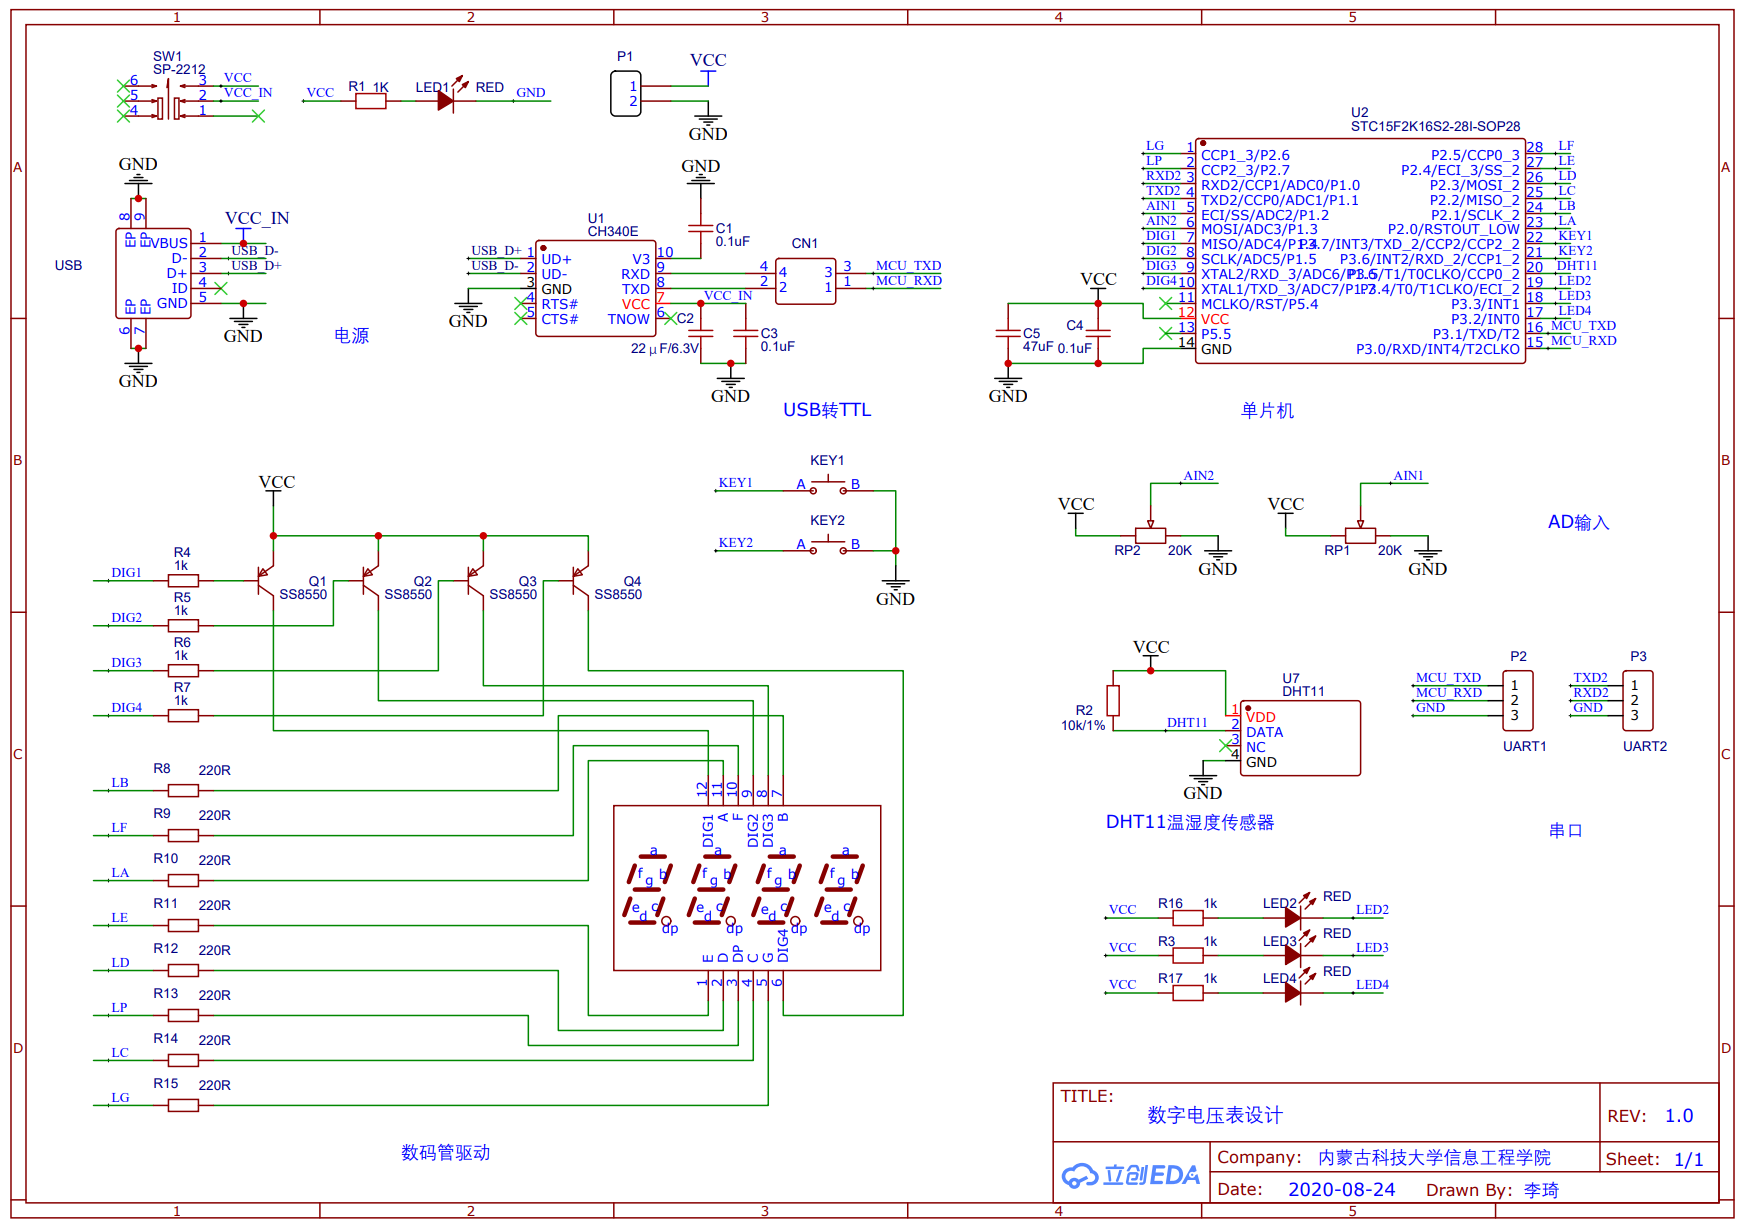
\includegraphics[width=\textwidth,angle=90]{figures/数字电压.png}
  \caption{单片机驱动四位数码管显示数字电压表电路原理图}
  \label{fig:5}
\end{figure}


\addtocontents{toc}{\protect\setcounter{tocdepth}{2}} % 恢复目录深度
\addcontentsline{toc}{chapter}{附录2}
\addtocontents{toc}{\protect\setcounter{tocdepth}{-1}} % 临时禁止加入目录
\chapter{}

这是一个关于数字电压表的源代码。这是一个关于数字电压表的源代码。这是一个关于数字电压表的源代码。这是一个关于数字电压表的源代码。这是一个关于数字电压表的源代码。这是一个关于数字电压表的源代码。

\begin{lstlisting}[language={[ANSI]C},extendedchars=false,tabsize=4, breaklines]
#include <reg51.h>
#include <intrins.h>
#include "common.h"
#define FOSC 11059200ul
#define T0_H (65536-(2*FOSC)/(1000*12))/256
#define T0_L (65536-(2*FOSC)/(1000*12))%256

sbit COM0 = P1^0;
sbit COM1 = P1^1;
sbit COM2 = P1^2;
sbit COM3 = P1^3;
sbit TLC549_CS = P1^6;
sbit TLC549_DOUT = P1^5;
sbit TLC549_CLK = P1^7;
bit flag = 0;
bit flag1 = 0;
uint8_t ADcounts = 0;
uint8_t dispBuf[] = { 2, 0, 1, 8};
uint8_t code ledDeg[] = { 0xC0, 0xF9, 0xA4, 0xB0, 0x99, 0x92, 0x82, 0xF8, 0x80, 0x90 };
uint8_t bdata AdValue;
sbit AIN = AdValue ^ 0;

void initSys();

uint8_t getAdValue() {
	uint8_t i;
	TLC549_CS = 0;
	TLC549_DOUT = 1;
	TLC549_CLK = 0;
	for (i = 0; i < 8; i++) {
		AdValue = AdValue << 1;
		TLC549_CLK = 1;
		_nop_();
		_nop_();
		AIN = TLC549_DOUT;
		TLC549_CLK = 0;
		_nop_();
		_nop_();
	}
	TLC549_CS = 1;
	return AdValue;
}

void main() {
	uint8_t i = 0;
	uint8_t j = 0;
	uint8_t ucAdValue = 0;
	uint16_t uiAdValue = 0;
	float fAdValue = 0.0;
	initSys();
	while (1) {
		if (flag1) {
			flag1 = 0;
			ucAdValue = getAdValue();
			fAdValue = (float)(ucAdValue * (5.0 / 255.0));
			uiAdValue = fAdValue * 1000;
			for (j = 0; j < 4; j++) {
				dispBuf[3 - j] = uiAdValue % 10;
				uiAdValue /= 10;
			}
		}
		if (flag) {
			flag = 0;
			switch (i) {
			case 0:
				COM0 = 0; COM1 = 1; COM2 = 1; COM3 = 1;
				break;
			case 1:
				COM0 = 1; COM1 = 0; COM2 = 1; COM3 = 1;
				break;
			case 2:
				COM0 = 1; COM1 = 1; COM2 = 0; COM3 = 1;
				break;
			case 3:
				COM0 = 1; COM1 = 1; COM2 = 1; COM3 = 0;
				break;
			}
			P3 = ledDeg[dispBuf[i]];
			if (i == 0)
				P3 &= 0x7f;
			if (++i >= 4)
				i = 0;
		}
	}
}

void initSys() {
	TMOD &= 0xF0;
	TMOD |= 0x01;
	EA = 1;
	ET0 = 1;
	TH0 = T0_H;
	TL0 = T0_L;
	TR0 = 1;
}

void timer0ISR()interrupt 1 {
	TH0 = T0_H;
	TL0 = T0_L;
	flag = 1;
	if (ADcounts++ >= 40) {
		ADcounts = 0;
		flag1 = 1;
	}
}
\end{lstlisting}  

\addtocontents{toc}{\protect\setcounter{tocdepth}{2}} % 恢复目录深度

%%%=========== 研究成果 ===========%%%-------------------------------------------
% !Mode:: "TeX:UTF-8"
% pages/acknowledgment.tex
%%%--- “攻读学位期间主要研究成果” --- %%%%%%%%%%%%%%%%%

\phantomsection
\titleformat{\chapter}{\centering\heiti\bfseries\zihao{3}}{}{1em}{}
\titlespacing{\chapter}{0pt}{-1em}{1em}
\addcontentsline{toc}{chapter}{攻读学位期间主要研究成果}
\markboth{攻读学位期间主要研究成果}{攻读学位期间主要研究成果}
\chapter*{攻读学位期间主要研究成果}

\noindent
一、	在学期间取得的科研成果

应注明课题名称、参加身份、通过时间、通过方式、评定单位等

\noindent
二、	在学期间所获的奖励

应注明奖励名称、授奖单位、授奖时间等

\noindent
三、	在学期间发表的论文

注： 应按照参考文献的格式来填写


\cleardoublepage
\end{document}



